\subsection{Experimental Setup}
\textit{Dataset.} The council was tested on 300 four-option questions from the test split of the Massive Multitask Language Understanding (MMLU) benchmark \cite{hendrycks2021mmlu}, 50 each from professional accounting and high-school macroeconomics (finance), jurisprudence and international law (law), and computer security and college computer science (technology). The questions were sampled once with a fixed seed (20261015) before any model was run, and none were used for tuning. Accuracy is the share of questions answered with the gold letter; chance is 25\%.

\textit{Models and runtime.} The pool contains seven instruction-tuned open-weight models of 1--1.7 billion parameters from seven developers (Table~\ref{tab:models}), each quantised to 4-bit (Q4\_K\_M) and served by llama.cpp \cite{llamacpp} on a 2-core CPU with 7\,GB of memory. Every call used temperature 0, one output token and the same prompt. $C_i$ in (\ref{eq:score}) is the model's probability for its chosen letter, renormalised over A--D from the top-20 token log-probabilities. Wall-clock latency and the token counts reported by the server were logged per call; prompt caching was disabled.

\textit{Configurations.} Each model answered every question once; council outcomes were then computed from these logged answers, so all configurations are compared on identical model outputs. The configurations are: the best single model; a round-robin single model (rotation without a council); all seven models; a fixed four-model council chosen a priori (the four largest models); the best of all 35 fixed four-model councils, selected on the test set and therefore optimistic; the rotational council of (\ref{eq:rot}) with four aggregation rules (Eq.~(\ref{eq:score}), plurality vote, confidence only and agreement only); and a uniformly random four-model council as the control for rotation. Rotational and random councils were run with ten seeds. Members were queried sequentially, so the parallel latency of a council is estimated as the slowest member's measured latency. Paired differences against the best single model use the exact McNemar test, and 95\% confidence intervals (CIs) use 10,000 bootstrap resamples of the questions.

\subsection{Single Models and Councils}
Table~\ref{tab:models} shows a wide spread in single-model accuracy. Qwen2.5-1.5B reached 57.7\%, Gemma-3-1B and Falcon3-1B about 43\%, and the other four models 28--29\%, close to chance. No call produced an invalid answer.

\begin{table}[t]
\caption{Single-Model Results on 300 MMLU Questions}
\label{tab:models}
\centering
\footnotesize
\setlength{\tabcolsep}{3.5pt}
\begin{tabular}{@{}lccccc@{}}
\toprule
Model & Acc. (\%) & 95\% CI & p50 (s) & p95 (s) & Tokens \\
\midrule
Qwen2.5-1.5B & 57.7 & 52.0--63.3 & 1.57 & 2.89 & 133 \\
Gemma-3-1B & 43.0 & 37.3--48.7 & 1.32 & 2.29 & 135 \\
Falcon3-1B & 42.7 & 37.0--48.3 & 1.42 & 2.26 & 144 \\
OLMo-2-1B & 28.7 & 23.7--34.0 & 1.25 & 1.98 & 134 \\
Llama-3.2-1B & 28.3 & 23.3--33.3 & 1.29 & 1.93 & 153 \\
SmolLM2-1.7B & 28.0 & 23.0--33.0 & 2.05 & 3.41 & 141 \\
Granite-3.1-1B & 27.7 & 22.7--32.7 & 0.84 & 1.33 & 145 \\
\bottomrule
\end{tabular}
\end{table}

Table~\ref{tab:council} and Fig.~\ref{fig:council} address whether the council improves accuracy. Against the average single model (36.6\%) or a round-robin single model (38.0\%), every council is better: the rotational council with (\ref{eq:score}) reached 44.6\% and the all-seven council 48.0\%. Against the best single model, no council is better. In each of the ten seeds the rotational council gained 19--25 questions over the best single model but lost 50--68 ($p\le0.001$ in every seed), and even the best fixed four-model council, picked with knowledge of the test answers, reached 54.3\% ($p=0.17$). The cost is four times the tokens (563 against 133 per query) and an estimated 3.00\,s parallel latency against 1.73\,s.

\begin{table}[t]
\caption{Council Configurations (Rot.\ = Rotational; Rotational and Random: Mean $\pm$ SD over 10 Seeds; $p$: McNemar Test Against the Best Single Model)}
\label{tab:council}
\centering
\footnotesize
\setlength{\tabcolsep}{2.6pt}
\begin{tabular}{@{}lccccc@{}}
\toprule
Configuration & Acc. (\%) & $p$ & Seq. (s) & Par. (s) & Tok. \\
\midrule
Best single (Qwen2.5) & 57.7 & -- & 1.73 & 1.73 & 133 \\
Round-robin single & 38.0 & $<$0.001 & 1.82 & 1.82 & 141 \\
All seven, Eq.~(\ref{eq:score}) & 48.0 & $<$0.001 & 11.80 & 3.71 & 985 \\
Fixed-4 a priori & 49.0 & 0.001 & 8.12 & 3.71 & 562 \\
Fixed-4 best (test) & 54.3 & 0.17 & 5.50 & 1.75 & 558 \\
Rot., Eq.~(\ref{eq:score}) & 44.6$\pm$1.7 & $\le$0.001 & 6.93 & 3.00 & 563 \\
Rot., plurality & 40.8$\pm$1.6 & $<$0.001 & 6.93 & 3.00 & 563 \\
Rot., confidence only & 48.1$\pm$1.9 & $\le$0.02 & 6.93 & 3.00 & 563 \\
Rot., agreement only & 40.5$\pm$2.8 & $<$0.001 & 6.93 & 3.00 & 563 \\
Random-4, Eq.~(\ref{eq:score}) & 45.0$\pm$2.5 & $\le$0.011 & 6.69 & 2.77 & 563 \\
Rot., quality-wtd.$^{*}$ & 51.0$\pm$2.6 & $\le$0.25 & -- & 2.61 & 559 \\
\bottomrule
\multicolumn{6}{@{}p{0.97\columnwidth}@{}}{\scriptsize $^{*}$Exploratory, added after the main results: $w_m$ in (\ref{eq:rot}) and vote weights set to each model's accuracy above chance on the other half of the questions (two-fold cross-fitting).}
\end{tabular}
\end{table}

\begin{figure}[t]
\centering
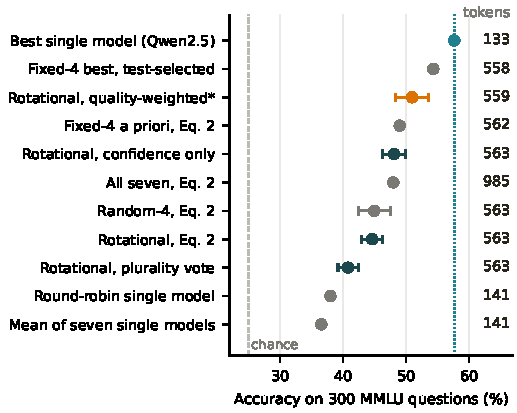
\includegraphics[width=\columnwidth]{figs/fig2_council.pdf}
\caption{Accuracy of single models and councils on the same 300 questions; bars show $\pm$1 SD over ten seeds, and the right column gives total tokens per query.}
\label{fig:council}
\end{figure}

The ablation isolates each part of the mechanism. Rotation itself adds no accuracy: rotational and random four-model councils differ by 0.4 points, well within their seed-to-seed spread. Its measurable effect is on load: over 300 queries no model waited more than 8 queries between selections under rotation, against 12 under random selection, while the spread of selection counts was the same (coefficient of variation 0.046 against 0.049). Within the consensus score, the agreement term is the harmful part. Agreement only (40.5\%) and plurality vote (40.8\%) are worse than confidence only (48.1\%), because the four near-chance models often agree on the same wrong option. Errors were only weakly correlated across models (mean pairwise correlation 0.16), and at least one of the seven models was right on 86.3\% of questions, so the information is in the pool; equal-weight agreement does not recover it. Weighting by held-out accuracy recovered part of the gap (51.0\%) but still lost to the best single model. This matches ensemble theory, in which voting helps when members are individually better than chance and comparably accurate \cite{dietterich2000ensemble}, and the finding that more calls can lower accuracy \cite{chen2024calls}.

\subsection{Deadlines and Member Failure}
Dropping members that miss a deadline bounds latency at the cost of accuracy. With the deadline set at the 90th percentile of single-call latency (2.19\,s), the council averaged 3.6 members, its 95th-percentile latency fell from 3.37\,s to 2.19\,s, and accuracy fell from 43.7\% to 42.7\% (seed 1); 4 of 300 queries returned no answer. A median deadline (1.37\,s) left two members on average, 54 unanswered queries and 33.7\% accuracy. When each member failed independently with probability 0.25 or 0.5, accuracy was 42.8\% and 39.7\% (10 seeds), so the council degrades gradually rather than failing outright.
